As described in the previous section, test methods are being developed that
will be suitable for comparing the performance of different kitting
planning systems. The methods look at plans that are an ordered sequence
of actions for a robot to perform. The actions are specified in terms of
the CRCL.

A sample plan file is shown in Figure~\ref{fig:KittingPlan}. The file is
designed for exercising the kittingViewer which is described in Section \ref{sect:KittingViewer}
and is not intended to make sense
as a plan. It includes a few intentional errors.

Metrics are being developed that will test both the static performance of the planning system
(i.e. end-to-end performance of a single plan without feedback or changes) as well as the
execution performance of the system (i.e. the system is allowed to replan due to changes
in the environment or action failures). The current metrics were developed with
kitting specifically in mind. However, it is envisioned that we will eventually have
a taxonomy of metrics where high-level metrics build upon lower level metrics and
branches of the taxonomy may be applicable across multiple domains. For many
applications, it will be useful to have a single numeric score that represents a system\rq{}s
performance with respect to the individual metrics. This may be accomplished by having a
user specify whether each weight is multiplicative or accumulative and specifying
weights for each of the accumulative metrics. The metric scores are then multiplied by
these weights and combined to form a single score that may be used for comparison.

\subsection{Static Kitting Viewer Metrics}
\begin{figure}[ht!]
		\begin{center}
			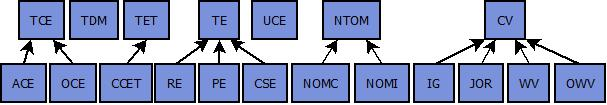
\includegraphics[width=3.1in]{images/MetricTaxonomy.jpg}
			%% Graphic for TeX using PGF
% Title: Z:\people\stephen\GlobalDocs\Projects\IPMAS\Architecture\Metric Taxonomy.dia
% Creator: Dia v0.97.2
% CreationDate: Thu Nov 01 16:39:04 2012
% For: stephen
% \usepackage{tikz}
% The following commands are not supported in PSTricks at present
% We define them conditionally, so when they are implemented,
% this pgf file will use them.
\ifx\du\undefined
  \newlength{\du}
\fi
\setlength{\du}{15\unitlength}
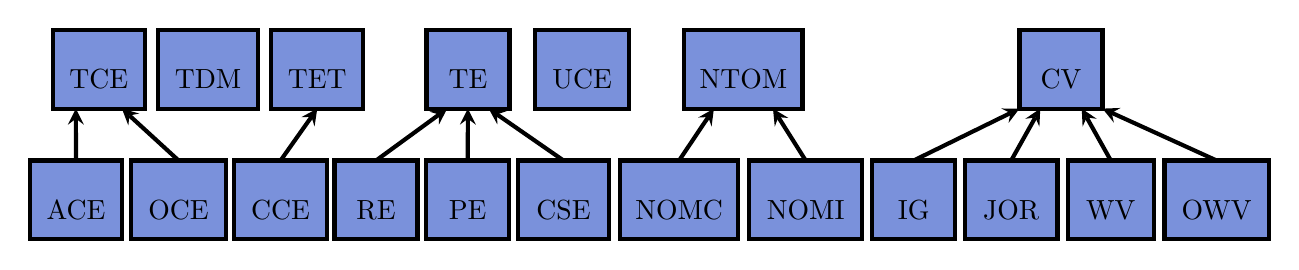
\begin{tikzpicture}
\pgftransformxscale{1.000000}
\pgftransformyscale{-1.000000}
\definecolor{dialinecolor}{rgb}{0.000000, 0.000000, 0.000000}
\pgfsetstrokecolor{dialinecolor}
\definecolor{dialinecolor}{rgb}{1.000000, 1.000000, 1.000000}
\pgfsetfillcolor{dialinecolor}
\definecolor{dialinecolor}{rgb}{0.478431, 0.568627, 0.858824}
\pgfsetfillcolor{dialinecolor}
\fill (1.257500\du,13.750000\du)--(1.257500\du,15.650000\du)--(3.487500\du,15.650000\du)--(3.487500\du,13.750000\du)--cycle;
\pgfsetlinewidth{0.100000\du}
\pgfsetdash{}{0pt}
\pgfsetdash{}{0pt}
\pgfsetmiterjoin
\definecolor{dialinecolor}{rgb}{0.000000, 0.000000, 0.000000}
\pgfsetstrokecolor{dialinecolor}
\draw (1.257500\du,13.750000\du)--(1.257500\du,15.650000\du)--(3.487500\du,15.650000\du)--(3.487500\du,13.750000\du)--cycle;
% setfont left to latex
\definecolor{dialinecolor}{rgb}{0.000000, 0.000000, 0.000000}
\pgfsetstrokecolor{dialinecolor}
\node at (2.372500\du,14.940000\du){ACE};
\definecolor{dialinecolor}{rgb}{0.478431, 0.568627, 0.858824}
\pgfsetfillcolor{dialinecolor}
\fill (3.694840\du,13.750000\du)--(3.694840\du,15.650000\du)--(5.992340\du,15.650000\du)--(5.992340\du,13.750000\du)--cycle;
\pgfsetlinewidth{0.100000\du}
\pgfsetdash{}{0pt}
\pgfsetdash{}{0pt}
\pgfsetmiterjoin
\definecolor{dialinecolor}{rgb}{0.000000, 0.000000, 0.000000}
\pgfsetstrokecolor{dialinecolor}
\draw (3.694840\du,13.750000\du)--(3.694840\du,15.650000\du)--(5.992340\du,15.650000\du)--(5.992340\du,13.750000\du)--cycle;
% setfont left to latex
\definecolor{dialinecolor}{rgb}{0.000000, 0.000000, 0.000000}
\pgfsetstrokecolor{dialinecolor}
\node at (4.843590\du,14.940000\du){OCE};
\definecolor{dialinecolor}{rgb}{0.478431, 0.568627, 0.858824}
\pgfsetfillcolor{dialinecolor}
\fill (1.812500\du,10.600000\du)--(1.812500\du,12.500000\du)--(4.032500\du,12.500000\du)--(4.032500\du,10.600000\du)--cycle;
\pgfsetlinewidth{0.100000\du}
\pgfsetdash{}{0pt}
\pgfsetdash{}{0pt}
\pgfsetmiterjoin
\definecolor{dialinecolor}{rgb}{0.000000, 0.000000, 0.000000}
\pgfsetstrokecolor{dialinecolor}
\draw (1.812500\du,10.600000\du)--(1.812500\du,12.500000\du)--(4.032500\du,12.500000\du)--(4.032500\du,10.600000\du)--cycle;
% setfont left to latex
\definecolor{dialinecolor}{rgb}{0.000000, 0.000000, 0.000000}
\pgfsetstrokecolor{dialinecolor}
\node at (2.922500\du,11.790000\du){TCE};
\definecolor{dialinecolor}{rgb}{0.478431, 0.568627, 0.858824}
\pgfsetfillcolor{dialinecolor}
\fill (4.352030\du,10.600000\du)--(4.352030\du,12.500000\du)--(6.754530\du,12.500000\du)--(6.754530\du,10.600000\du)--cycle;
\pgfsetlinewidth{0.100000\du}
\pgfsetdash{}{0pt}
\pgfsetdash{}{0pt}
\pgfsetmiterjoin
\definecolor{dialinecolor}{rgb}{0.000000, 0.000000, 0.000000}
\pgfsetstrokecolor{dialinecolor}
\draw (4.352030\du,10.600000\du)--(4.352030\du,12.500000\du)--(6.754530\du,12.500000\du)--(6.754530\du,10.600000\du)--cycle;
% setfont left to latex
\definecolor{dialinecolor}{rgb}{0.000000, 0.000000, 0.000000}
\pgfsetstrokecolor{dialinecolor}
\node at (5.553280\du,11.790000\du){TDM};
\definecolor{dialinecolor}{rgb}{0.478431, 0.568627, 0.858824}
\pgfsetfillcolor{dialinecolor}
\fill (7.074060\du,10.600000\du)--(7.074060\du,12.500000\du)--(9.294060\du,12.500000\du)--(9.294060\du,10.600000\du)--cycle;
\pgfsetlinewidth{0.100000\du}
\pgfsetdash{}{0pt}
\pgfsetdash{}{0pt}
\pgfsetmiterjoin
\definecolor{dialinecolor}{rgb}{0.000000, 0.000000, 0.000000}
\pgfsetstrokecolor{dialinecolor}
\draw (7.074060\du,10.600000\du)--(7.074060\du,12.500000\du)--(9.294060\du,12.500000\du)--(9.294060\du,10.600000\du)--cycle;
% setfont left to latex
\definecolor{dialinecolor}{rgb}{0.000000, 0.000000, 0.000000}
\pgfsetstrokecolor{dialinecolor}
\node at (8.184060\du,11.790000\du){TET};
\definecolor{dialinecolor}{rgb}{0.478431, 0.568627, 0.858824}
\pgfsetfillcolor{dialinecolor}
\fill (8.599690\du,13.750000\du)--(8.599690\du,15.650000\du)--(10.599690\du,15.650000\du)--(10.599690\du,13.750000\du)--cycle;
\pgfsetlinewidth{0.100000\du}
\pgfsetdash{}{0pt}
\pgfsetdash{}{0pt}
\pgfsetmiterjoin
\definecolor{dialinecolor}{rgb}{0.000000, 0.000000, 0.000000}
\pgfsetstrokecolor{dialinecolor}
\draw (8.599690\du,13.750000\du)--(8.599690\du,15.650000\du)--(10.599690\du,15.650000\du)--(10.599690\du,13.750000\du)--cycle;
% setfont left to latex
\definecolor{dialinecolor}{rgb}{0.000000, 0.000000, 0.000000}
\pgfsetstrokecolor{dialinecolor}
\node at (9.599690\du,14.940000\du){RE};
\definecolor{dialinecolor}{rgb}{0.478431, 0.568627, 0.858824}
\pgfsetfillcolor{dialinecolor}
\fill (10.807000\du,13.750000\du)--(10.807000\du,15.650000\du)--(12.807000\du,15.650000\du)--(12.807000\du,13.750000\du)--cycle;
\pgfsetlinewidth{0.100000\du}
\pgfsetdash{}{0pt}
\pgfsetdash{}{0pt}
\pgfsetmiterjoin
\definecolor{dialinecolor}{rgb}{0.000000, 0.000000, 0.000000}
\pgfsetstrokecolor{dialinecolor}
\draw (10.807000\du,13.750000\du)--(10.807000\du,15.650000\du)--(12.807000\du,15.650000\du)--(12.807000\du,13.750000\du)--cycle;
% setfont left to latex
\definecolor{dialinecolor}{rgb}{0.000000, 0.000000, 0.000000}
\pgfsetstrokecolor{dialinecolor}
\node at (11.807000\du,14.940000\du){PE};
\definecolor{dialinecolor}{rgb}{0.478431, 0.568627, 0.858824}
\pgfsetfillcolor{dialinecolor}
\fill (13.014400\du,13.750000\du)--(13.014400\du,15.650000\du)--(15.216900\du,15.650000\du)--(15.216900\du,13.750000\du)--cycle;
\pgfsetlinewidth{0.100000\du}
\pgfsetdash{}{0pt}
\pgfsetdash{}{0pt}
\pgfsetmiterjoin
\definecolor{dialinecolor}{rgb}{0.000000, 0.000000, 0.000000}
\pgfsetstrokecolor{dialinecolor}
\draw (13.014400\du,13.750000\du)--(13.014400\du,15.650000\du)--(15.216900\du,15.650000\du)--(15.216900\du,13.750000\du)--cycle;
% setfont left to latex
\definecolor{dialinecolor}{rgb}{0.000000, 0.000000, 0.000000}
\pgfsetstrokecolor{dialinecolor}
\node at (14.115650\du,14.940000\du){CSE};
\definecolor{dialinecolor}{rgb}{0.478431, 0.568627, 0.858824}
\pgfsetfillcolor{dialinecolor}
\fill (10.813600\du,10.600000\du)--(10.813600\du,12.500000\du)--(12.813600\du,12.500000\du)--(12.813600\du,10.600000\du)--cycle;
\pgfsetlinewidth{0.100000\du}
\pgfsetdash{}{0pt}
\pgfsetdash{}{0pt}
\pgfsetmiterjoin
\definecolor{dialinecolor}{rgb}{0.000000, 0.000000, 0.000000}
\pgfsetstrokecolor{dialinecolor}
\draw (10.813600\du,10.600000\du)--(10.813600\du,12.500000\du)--(12.813600\du,12.500000\du)--(12.813600\du,10.600000\du)--cycle;
% setfont left to latex
\definecolor{dialinecolor}{rgb}{0.000000, 0.000000, 0.000000}
\pgfsetstrokecolor{dialinecolor}
\node at (11.813600\du,11.790000\du){TE};
\definecolor{dialinecolor}{rgb}{0.478431, 0.568627, 0.858824}
\pgfsetfillcolor{dialinecolor}
\fill (13.433100\du,10.600000\du)--(13.433100\du,12.500000\du)--(15.698100\du,12.500000\du)--(15.698100\du,10.600000\du)--cycle;
\pgfsetlinewidth{0.100000\du}
\pgfsetdash{}{0pt}
\pgfsetdash{}{0pt}
\pgfsetmiterjoin
\definecolor{dialinecolor}{rgb}{0.000000, 0.000000, 0.000000}
\pgfsetstrokecolor{dialinecolor}
\draw (13.433100\du,10.600000\du)--(13.433100\du,12.500000\du)--(15.698100\du,12.500000\du)--(15.698100\du,10.600000\du)--cycle;
% setfont left to latex
\definecolor{dialinecolor}{rgb}{0.000000, 0.000000, 0.000000}
\pgfsetstrokecolor{dialinecolor}
\node at (14.565600\du,11.790000\du){UCE};
\pgfsetlinewidth{0.100000\du}
\pgfsetdash{}{0pt}
\pgfsetdash{}{0pt}
\pgfsetbuttcap
{
\definecolor{dialinecolor}{rgb}{0.000000, 0.000000, 0.000000}
\pgfsetfillcolor{dialinecolor}
% was here!!!
\pgfsetarrowsend{stealth}
\definecolor{dialinecolor}{rgb}{0.000000, 0.000000, 0.000000}
\pgfsetstrokecolor{dialinecolor}
\draw (2.372500\du,13.750000\du)--(2.367500\du,12.500000\du);
}
\pgfsetlinewidth{0.100000\du}
\pgfsetdash{}{0pt}
\pgfsetdash{}{0pt}
\pgfsetbuttcap
{
\definecolor{dialinecolor}{rgb}{0.000000, 0.000000, 0.000000}
\pgfsetfillcolor{dialinecolor}
% was here!!!
\pgfsetarrowsend{stealth}
\definecolor{dialinecolor}{rgb}{0.000000, 0.000000, 0.000000}
\pgfsetstrokecolor{dialinecolor}
\draw (4.843590\du,13.750000\du)--(3.477500\du,12.500000\du);
}
\pgfsetlinewidth{0.100000\du}
\pgfsetdash{}{0pt}
\pgfsetdash{}{0pt}
\pgfsetbuttcap
{
\definecolor{dialinecolor}{rgb}{0.000000, 0.000000, 0.000000}
\pgfsetfillcolor{dialinecolor}
% was here!!!
\pgfsetarrowsend{stealth}
\definecolor{dialinecolor}{rgb}{0.000000, 0.000000, 0.000000}
\pgfsetstrokecolor{dialinecolor}
\draw (9.599690\du,13.750000\du)--(11.313600\du,12.500000\du);
}
\pgfsetlinewidth{0.100000\du}
\pgfsetdash{}{0pt}
\pgfsetdash{}{0pt}
\pgfsetbuttcap
{
\definecolor{dialinecolor}{rgb}{0.000000, 0.000000, 0.000000}
\pgfsetfillcolor{dialinecolor}
% was here!!!
\pgfsetarrowsend{stealth}
\definecolor{dialinecolor}{rgb}{0.000000, 0.000000, 0.000000}
\pgfsetstrokecolor{dialinecolor}
\draw (11.807000\du,13.750000\du)--(11.813600\du,12.500000\du);
}
\pgfsetlinewidth{0.100000\du}
\pgfsetdash{}{0pt}
\pgfsetdash{}{0pt}
\pgfsetbuttcap
{
\definecolor{dialinecolor}{rgb}{0.000000, 0.000000, 0.000000}
\pgfsetfillcolor{dialinecolor}
% was here!!!
\pgfsetarrowsend{stealth}
\definecolor{dialinecolor}{rgb}{0.000000, 0.000000, 0.000000}
\pgfsetstrokecolor{dialinecolor}
\draw (14.115650\du,13.750000\du)--(12.313600\du,12.500000\du);
}
\definecolor{dialinecolor}{rgb}{0.478431, 0.568627, 0.858824}
\pgfsetfillcolor{dialinecolor}
\fill (6.185000\du,13.750000\du)--(6.185000\du,15.650000\du)--(8.415000\du,15.650000\du)--(8.415000\du,13.750000\du)--cycle;
\pgfsetlinewidth{0.100000\du}
\pgfsetdash{}{0pt}
\pgfsetdash{}{0pt}
\pgfsetmiterjoin
\definecolor{dialinecolor}{rgb}{0.000000, 0.000000, 0.000000}
\pgfsetstrokecolor{dialinecolor}
\draw (6.185000\du,13.750000\du)--(6.185000\du,15.650000\du)--(8.415000\du,15.650000\du)--(8.415000\du,13.750000\du)--cycle;
% setfont left to latex
\definecolor{dialinecolor}{rgb}{0.000000, 0.000000, 0.000000}
\pgfsetstrokecolor{dialinecolor}
\node at (7.300000\du,14.940000\du){CCE};
\pgfsetlinewidth{0.100000\du}
\pgfsetdash{}{0pt}
\pgfsetdash{}{0pt}
\pgfsetbuttcap
{
\definecolor{dialinecolor}{rgb}{0.000000, 0.000000, 0.000000}
\pgfsetfillcolor{dialinecolor}
% was here!!!
\pgfsetarrowsend{stealth}
\definecolor{dialinecolor}{rgb}{0.000000, 0.000000, 0.000000}
\pgfsetstrokecolor{dialinecolor}
\draw (7.300000\du,13.750000\du)--(8.184060\du,12.500000\du);
}
\definecolor{dialinecolor}{rgb}{0.478431, 0.568627, 0.858824}
\pgfsetfillcolor{dialinecolor}
\fill (15.471250\du,13.750000\du)--(15.471250\du,15.650000\du)--(18.328750\du,15.650000\du)--(18.328750\du,13.750000\du)--cycle;
\pgfsetlinewidth{0.100000\du}
\pgfsetdash{}{0pt}
\pgfsetdash{}{0pt}
\pgfsetmiterjoin
\definecolor{dialinecolor}{rgb}{0.000000, 0.000000, 0.000000}
\pgfsetstrokecolor{dialinecolor}
\draw (15.471250\du,13.750000\du)--(15.471250\du,15.650000\du)--(18.328750\du,15.650000\du)--(18.328750\du,13.750000\du)--cycle;
% setfont left to latex
\definecolor{dialinecolor}{rgb}{0.000000, 0.000000, 0.000000}
\pgfsetstrokecolor{dialinecolor}
\node at (16.900000\du,14.940000\du){NOMC};
\definecolor{dialinecolor}{rgb}{0.478431, 0.568627, 0.858824}
\pgfsetfillcolor{dialinecolor}
\fill (18.593750\du,13.750000\du)--(18.593750\du,15.650000\du)--(21.306250\du,15.650000\du)--(21.306250\du,13.750000\du)--cycle;
\pgfsetlinewidth{0.100000\du}
\pgfsetdash{}{0pt}
\pgfsetdash{}{0pt}
\pgfsetmiterjoin
\definecolor{dialinecolor}{rgb}{0.000000, 0.000000, 0.000000}
\pgfsetstrokecolor{dialinecolor}
\draw (18.593750\du,13.750000\du)--(18.593750\du,15.650000\du)--(21.306250\du,15.650000\du)--(21.306250\du,13.750000\du)--cycle;
% setfont left to latex
\definecolor{dialinecolor}{rgb}{0.000000, 0.000000, 0.000000}
\pgfsetstrokecolor{dialinecolor}
\node at (19.950000\du,14.940000\du){NOMI};
\definecolor{dialinecolor}{rgb}{0.478431, 0.568627, 0.858824}
\pgfsetfillcolor{dialinecolor}
\fill (17.026250\du,10.600000\du)--(17.026250\du,12.500000\du)--(19.873750\du,12.500000\du)--(19.873750\du,10.600000\du)--cycle;
\pgfsetlinewidth{0.100000\du}
\pgfsetdash{}{0pt}
\pgfsetdash{}{0pt}
\pgfsetmiterjoin
\definecolor{dialinecolor}{rgb}{0.000000, 0.000000, 0.000000}
\pgfsetstrokecolor{dialinecolor}
\draw (17.026250\du,10.600000\du)--(17.026250\du,12.500000\du)--(19.873750\du,12.500000\du)--(19.873750\du,10.600000\du)--cycle;
% setfont left to latex
\definecolor{dialinecolor}{rgb}{0.000000, 0.000000, 0.000000}
\pgfsetstrokecolor{dialinecolor}
\node at (18.450000\du,11.790000\du){NTOM};
\definecolor{dialinecolor}{rgb}{0.478431, 0.568627, 0.858824}
\pgfsetfillcolor{dialinecolor}
\fill (21.550000\du,13.750000\du)--(21.550000\du,15.650000\du)--(23.550000\du,15.650000\du)--(23.550000\du,13.750000\du)--cycle;
\pgfsetlinewidth{0.100000\du}
\pgfsetdash{}{0pt}
\pgfsetdash{}{0pt}
\pgfsetmiterjoin
\definecolor{dialinecolor}{rgb}{0.000000, 0.000000, 0.000000}
\pgfsetstrokecolor{dialinecolor}
\draw (21.550000\du,13.750000\du)--(21.550000\du,15.650000\du)--(23.550000\du,15.650000\du)--(23.550000\du,13.750000\du)--cycle;
% setfont left to latex
\definecolor{dialinecolor}{rgb}{0.000000, 0.000000, 0.000000}
\pgfsetstrokecolor{dialinecolor}
\node at (22.550000\du,14.940000\du){IG};
\definecolor{dialinecolor}{rgb}{0.478431, 0.568627, 0.858824}
\pgfsetfillcolor{dialinecolor}
\fill (23.783750\du,13.750000\du)--(23.783750\du,15.650000\du)--(26.016250\du,15.650000\du)--(26.016250\du,13.750000\du)--cycle;
\pgfsetlinewidth{0.100000\du}
\pgfsetdash{}{0pt}
\pgfsetdash{}{0pt}
\pgfsetmiterjoin
\definecolor{dialinecolor}{rgb}{0.000000, 0.000000, 0.000000}
\pgfsetstrokecolor{dialinecolor}
\draw (23.783750\du,13.750000\du)--(23.783750\du,15.650000\du)--(26.016250\du,15.650000\du)--(26.016250\du,13.750000\du)--cycle;
% setfont left to latex
\definecolor{dialinecolor}{rgb}{0.000000, 0.000000, 0.000000}
\pgfsetstrokecolor{dialinecolor}
\node at (24.900000\du,14.940000\du){JOR};
\definecolor{dialinecolor}{rgb}{0.478431, 0.568627, 0.858824}
\pgfsetfillcolor{dialinecolor}
\fill (26.268750\du,13.750000\du)--(26.268750\du,15.650000\du)--(28.331250\du,15.650000\du)--(28.331250\du,13.750000\du)--cycle;
\pgfsetlinewidth{0.100000\du}
\pgfsetdash{}{0pt}
\pgfsetdash{}{0pt}
\pgfsetmiterjoin
\definecolor{dialinecolor}{rgb}{0.000000, 0.000000, 0.000000}
\pgfsetstrokecolor{dialinecolor}
\draw (26.268750\du,13.750000\du)--(26.268750\du,15.650000\du)--(28.331250\du,15.650000\du)--(28.331250\du,13.750000\du)--cycle;
% setfont left to latex
\definecolor{dialinecolor}{rgb}{0.000000, 0.000000, 0.000000}
\pgfsetstrokecolor{dialinecolor}
\node at (27.300000\du,14.940000\du){WV};
\definecolor{dialinecolor}{rgb}{0.478431, 0.568627, 0.858824}
\pgfsetfillcolor{dialinecolor}
\fill (28.593750\du,13.750000\du)--(28.593750\du,15.650000\du)--(31.106250\du,15.650000\du)--(31.106250\du,13.750000\du)--cycle;
\pgfsetlinewidth{0.100000\du}
\pgfsetdash{}{0pt}
\pgfsetdash{}{0pt}
\pgfsetmiterjoin
\definecolor{dialinecolor}{rgb}{0.000000, 0.000000, 0.000000}
\pgfsetstrokecolor{dialinecolor}
\draw (28.593750\du,13.750000\du)--(28.593750\du,15.650000\du)--(31.106250\du,15.650000\du)--(31.106250\du,13.750000\du)--cycle;
% setfont left to latex
\definecolor{dialinecolor}{rgb}{0.000000, 0.000000, 0.000000}
\pgfsetstrokecolor{dialinecolor}
\node at (29.850000\du,14.940000\du){OWV};
\definecolor{dialinecolor}{rgb}{0.478431, 0.568627, 0.858824}
\pgfsetfillcolor{dialinecolor}
\fill (25.100000\du,10.600000\du)--(25.100000\du,12.500000\du)--(27.100000\du,12.500000\du)--(27.100000\du,10.600000\du)--cycle;
\pgfsetlinewidth{0.100000\du}
\pgfsetdash{}{0pt}
\pgfsetdash{}{0pt}
\pgfsetmiterjoin
\definecolor{dialinecolor}{rgb}{0.000000, 0.000000, 0.000000}
\pgfsetstrokecolor{dialinecolor}
\draw (25.100000\du,10.600000\du)--(25.100000\du,12.500000\du)--(27.100000\du,12.500000\du)--(27.100000\du,10.600000\du)--cycle;
% setfont left to latex
\definecolor{dialinecolor}{rgb}{0.000000, 0.000000, 0.000000}
\pgfsetstrokecolor{dialinecolor}
\node at (26.100000\du,11.790000\du){CV};
\pgfsetlinewidth{0.100000\du}
\pgfsetdash{}{0pt}
\pgfsetdash{}{0pt}
\pgfsetbuttcap
{
\definecolor{dialinecolor}{rgb}{0.000000, 0.000000, 0.000000}
\pgfsetfillcolor{dialinecolor}
% was here!!!
\pgfsetarrowsend{stealth}
\definecolor{dialinecolor}{rgb}{0.000000, 0.000000, 0.000000}
\pgfsetstrokecolor{dialinecolor}
\draw (16.900000\du,13.750000\du)--(17.738125\du,12.500000\du);
}
\pgfsetlinewidth{0.100000\du}
\pgfsetdash{}{0pt}
\pgfsetdash{}{0pt}
\pgfsetbuttcap
{
\definecolor{dialinecolor}{rgb}{0.000000, 0.000000, 0.000000}
\pgfsetfillcolor{dialinecolor}
% was here!!!
\pgfsetarrowsend{stealth}
\definecolor{dialinecolor}{rgb}{0.000000, 0.000000, 0.000000}
\pgfsetstrokecolor{dialinecolor}
\draw (19.950000\du,13.750000\du)--(19.161875\du,12.500000\du);
}
\pgfsetlinewidth{0.100000\du}
\pgfsetdash{}{0pt}
\pgfsetdash{}{0pt}
\pgfsetbuttcap
{
\definecolor{dialinecolor}{rgb}{0.000000, 0.000000, 0.000000}
\pgfsetfillcolor{dialinecolor}
% was here!!!
\pgfsetarrowsend{stealth}
\definecolor{dialinecolor}{rgb}{0.000000, 0.000000, 0.000000}
\pgfsetstrokecolor{dialinecolor}
\draw (22.550000\du,13.750000\du)--(25.100000\du,12.500000\du);
}
\pgfsetlinewidth{0.100000\du}
\pgfsetdash{}{0pt}
\pgfsetdash{}{0pt}
\pgfsetbuttcap
{
\definecolor{dialinecolor}{rgb}{0.000000, 0.000000, 0.000000}
\pgfsetfillcolor{dialinecolor}
% was here!!!
\pgfsetarrowsend{stealth}
\definecolor{dialinecolor}{rgb}{0.000000, 0.000000, 0.000000}
\pgfsetstrokecolor{dialinecolor}
\draw (24.900000\du,13.750000\du)--(25.600000\du,12.500000\du);
}
\pgfsetlinewidth{0.100000\du}
\pgfsetdash{}{0pt}
\pgfsetdash{}{0pt}
\pgfsetbuttcap
{
\definecolor{dialinecolor}{rgb}{0.000000, 0.000000, 0.000000}
\pgfsetfillcolor{dialinecolor}
% was here!!!
\pgfsetarrowsend{stealth}
\definecolor{dialinecolor}{rgb}{0.000000, 0.000000, 0.000000}
\pgfsetstrokecolor{dialinecolor}
\draw (27.300000\du,13.750000\du)--(26.600000\du,12.500000\du);
}
\pgfsetlinewidth{0.100000\du}
\pgfsetdash{}{0pt}
\pgfsetdash{}{0pt}
\pgfsetbuttcap
{
\definecolor{dialinecolor}{rgb}{0.000000, 0.000000, 0.000000}
\pgfsetfillcolor{dialinecolor}
% was here!!!
\pgfsetarrowsend{stealth}
\definecolor{dialinecolor}{rgb}{0.000000, 0.000000, 0.000000}
\pgfsetstrokecolor{dialinecolor}
\draw (29.850000\du,13.750000\du)--(27.100000\du,12.500000\du);
}
\end{tikzpicture}
}
		\end{center}

	\caption{Kitting static metric taxonomy with abbreviations defined below}
	\label{fig:StaticMetricTax}
\end{figure}

The current metric taxonomy is shown in Figure~\ref{fig:StaticMetricTax} and is
described below. The metrics are designed to be evaluated at the end of each
CRCL command with cumulative values.

\begin{itemize}

\item \sf Action Commands Executed (ACE) \rm -- the number of action commands that
  have been executed so far. An action command is any command that takes
  time to execute.\\

\item \sf Command Sequence Errors (CSE) \rm -- the number of commands that are
  out of sequence. An InitCanon command is out of sequence if it is not the
  first command in the file. An EndCanon command is out of sequence if it
  is not the last command in the file. Other commands are out of sequence
  if they occur before InitCanon or after EndCanon.\\

\item \sf Constraint Violations (CV) \rm -- the total of IG, JOR, WV and OWV.\\

\item \sf Current Command Execution Time (CCET) \rm -- the time that the current
   command took to execute.\\

\item \sf Incorrect Gripper (IG) \rm -- the wrong gripper was used to pick up an object.\\

\item \sf Joint Out of Range (JOR) \rm -- a joint of the robot was commanded to
  move to an out-of-limit position.\\

\item \sf Number of Objects Moved Correctly (NOMC) \rm -- the number of objects
  that were moved correctly from the parts supply to the kit.\\

\item \sf Number of Objects Moved Incorrectly (NOMI) \rm -- the number of objects
  that were moved to an incorrect position in the kit.\\

\item \sf Number of Total Objects Moved (NTOM) \rm -- the sum of NOMC and NOMI.\\

\item \sf Other Commands Executed (OCE) \rm -- the number of commands that are
  not action commands that have been executed so far -- mostly setting
  commands. Executing these commands is assumed to take a negligible amount
  of time.\\

\item \sf Outside Work Volume (OWV) \rm -- the robot was asked to move outside its
  work volume.\\

\item \sf Parse Errors  (PE) \rm -- the number of lines in the CRCL command file
  that cause an error in the command file parser. \\

\item \sf Range Errors (RE) \rm -- the number of times a command tries to set a
  a parameter to a value that is out of the allowed range of the parameter.\\

 \item \sf Total Commands Executed (TCE) \rm -- the sum of ACE and OCE.\\

\item \sf Total Distance Moved (TDM) \rm -- the total distance that the
  tool tip has moved.  This is calculated as the total of the distances between
  points in
  the move commands, taken in order (and starting at the place where the
  controlled point is located initially). The value is updated as each point
  is reached, not continuously.\\

\item \sf Total Execution Time (TET) \rm -- the total time taken so far by
  executing action commands. This does not include any time that may elapse
  between when one command finishes execution and when the user tells the
  system to execute another command. The total execution time is
  meant to be very close to the actual amount of time that would be taken
  by the system without user intervention.\\

\item \sf Total Errors (TE) \rm -- the sum of the range errors, parse errors,
  and command sequence errors.\\

\item \sf Useless Command Executed (UCE) \rm -- the number of commands that do
  not change the state of the workstation. Such commands have no effect, so
  they are useless. The \sf CloseGripper() \rm and \sf CloseToolChanger()
  \rm commands in Figure~\ref{fig:KittingPlan} are useless because the
  gripper and tool changer are closed in the initial conditions.\\

\item \sf Weight Violation (WV) \rm -- the robot was asked to move some object that
  violates its load capacity.

\end{itemize}

\subsection{Execution Metrics for Kit Building}
During execution, automated kitting fails to reach its full potential when the supply chain fails and parts and components are not available for kit construction, or when a kit is not properly filled. Part availability failures can be triggered by inaccurate information about the location of the part or part shortage due to delays in internal logistics. Kit construction errors may be due to problems such as improper equipment setup, improper equipment maintenance, part damage, wrong type of part, or part dropped by the robot.


Models for detecting and recovering from plan execution failures mostly deal with \textit{precondition failures}, \textit{action failures}, and \textit{unattributable failures}~\cite{Myers1998}. Precondition failures appear when all the preconditions for an action are not met during the execution of the action. Action failures are encountered when the execution of an action does not attain its intended effects. Unattributable failures occur when unexpected events caused by external agents change the environment, thus causing the current plan to become obsolete. NIST\rq{}s Knowledge Driven Planning and Modeling project has not yet addressed the creation of a taxonomy of  execution errors. However, some preliminary metrics have been developed and are described
below.

\begin{itemize}
\item \sf Manipulation robustness \rm -- quantitative and qualitative functionality metrics that describe how well a robot can handle complex objects in complex environments without failing or requiring additional operator interventions. Failures can occur during object detection (lightning variation, shadows), object approach (partially buried), and object manipulation (fragile) operations.
It is envisioned that a taxonomy of robustness will be developed that decomposes robustness into areas such as situational awareness, robot accuracy, and grasping dexterity.\\

\item \sf Transporting components \rm -- qualitative metrics that describe how well a robotic arm can grasp objects and move these objects from an initial position to a goal position without dropping them.\\

\item \sf Plan generation \rm -- as mentioned previously, failures are possible in kitting during the execution of CRCL commands, causing the current plan to become obsolete. In some cases, the current state of the environment is brought back to the state prior to the failure and the robot starts from a ``stable" state. In other cases, a completely new plan must be generated by the planning system where the robot starts all over. This metric will measure the planning system\rq{}s ability to adapt to failures.\\

\item \sf Contact errors \rm -- quantitative metrics that keep track of the number of collisions between the robotic arm and objects in the environment. The performance of the robotic arm during kit building is affected by the positions of joints and the end-effector in the environment. The position of the end-effector can reduce the time to complete tasks but can also increase the number of collisions due to joint contact with other objects in a confined space.\\

\item \sf Failures during kit building\rm -- quantitative metrics that report the total number of failures encountered during kit building. When a failure occurs during the
building of a kit, the number of failures is increased by one. The system may generate a new plan to recover from the failure. If a failure occurs during the execution of the new
plan, the number of failures in increased by one again.\\

\item \sf Failure modes recovery \rm -- quantitative metrics that represent the number of failure modes the system recovers from through the use of contingency plans. When a failure is detected in the execution process, failure monitors encode appropriate responses (contingency plans) to failure modes for this particular failure.\\

\end{itemize}
